\documentclass{template/openetcs_article}
% Use the option "nocc" if the document is not licensed under Creative Commons
%\documentclass[nocc]{template/openetcs_article}
\usepackage {bsymb,b2latex}
\usepackage{lipsum,url,color}
\graphicspath{{./template/}{.}{./images/}}
\begin{document}
\frontmatter
\project{openETCS}

%Please do not change anything above this line
%============================
% The document metadata is defined below

%assign a report number here
\reportnum{OETCS}

%define your workpackage here
\wp{Work-Package 7: ``Toolchain''}


\newcommand{\true}{\ensuremath{true}}
\newcommand{\btext}[1]{{\it #1}}
\newcommand{\bvar}[1]{\btext{#1}}
\newcommand{\bevent}[1]{\btext{#1}}
\newcommand{\binv}[1]{\btext{#1}}
\newcommand{\bconst}[1]{\btext{#1}}
\newcommand{\bparam}[1]{\btext{#1}}
\newcommand{\bfunc}[1]{\btext{#1}}
\newcommand{\baxiom}[1]{\btext{#1}}
\newcommand{\btype}[1]{\btext{#1}}
\newcommand{\bguard}[1]{\btext{#1}}
\newcommand{\bmachine}[1]{\btext{#1}}
\newcommand{\bctx}[1]{\btext{#1}}

\author{Matthias Güdemann}

\affiliation{Systerel\\
  Les Portes de l’Arbois, Bâtiment A \\
  1090 rue René Descartes \\
  13857 Aix-en-Provence Cedex 3, France
}

\title{Event-B Model of Subset 026, Section 3.13}

% define the coverart
\coverart[width=350pt]{openETCS_EUPL}

\reporttype{Model Description}

%\begin{document}

\maketitle
\tableofcontents
\listoffiguresandtables
\newpage

This document describes a formal model of the requirements of section~3.13 of
the subset 026 of the ETCS specification 3.3.0~\cite{SRS-026-330}. This section
describes the speed and distance monitoring subsystem of ETCS.

The model is expressed in the formal language Event-B~\cite{abrial-eventB-Book}
and developed within the Rodin tool~\cite{rodin-handbook}. This formalism allows
an iterative modeling approach. In general, one starts with a very abstract
description of the basic functionality and step-wise adds additional details
until the desired level of accuracy of the model is reached. Rodin provides the
necessary proof support to ensure the correctness of the refined behavior.

In this document we present an Event-B model of the speed and distance
monitoring subsystem of ETCS. At first, we describe shortly the background of
Event-B, then the overall approach taken to model this section and finally
present the model in detail.

The section~3.13 of the SRS gives a very detailed description of the calculation
of many necessary values for speed and distance monitoring. As Event-B is a
system modeling approach, we give an abstract model of the system. The
calculations are abstracted as functions and the system ensures the correct
parameter flow to the functions. We illustrate the model decomposition
capabilities of Event-B and Rodin by decomposing the overall model into
different functional parts.

For a short introduction on Event-B and the usage of Rodin with models on github
see~\url{https://github.com/openETCS/model-evaluation/blob/master/model/B-Systerel/Event_B/rodin-projects-github.pdf?raw=true}

% \begin{table}[ht]
%   \centering
%   \begin{tabular}[ht]{|l|l|}
%     \hline
%      &  \\
%     \hline
%   \end{tabular}
%   \caption{Glossary}
%   \label{tab:glossary}
% \end{table}

\section{Modeling Strategy}
\label{sec:modeling-strategy}

The section~3.13 of the SRS describes the speed and distance monitoring together
with the necessary parameters and data. The model starts with an abstract
modeling of dataflow of the various intermediate calculated values. This model
is partitioned into functional parts, the model is decomposed using shared
variables and the respective sub-models are refined until the basic calculation
functions are reached.

\section{Model Overview}
\label{sec:model-overview}

The overview of the speed and distance monitoring is shown in
Fig.~\ref{fig:speed-distance-system} from the SRS.

\begin{figure}[ht]
  \centering
  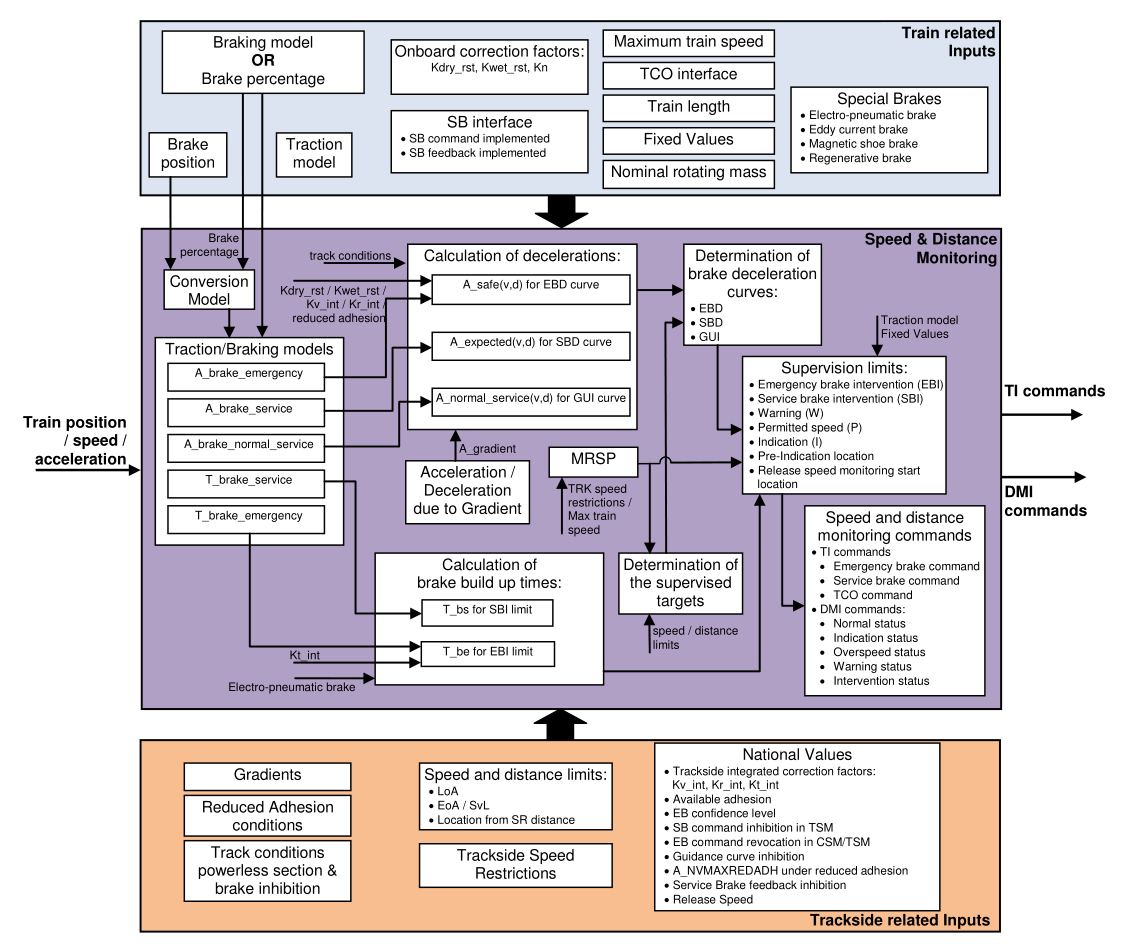
\includegraphics[width=.9\textwidth]{Overview_13_3}
  \caption{Speed and Distance Monitoring Overview~(\cite{SRS-026-330}~p.~85)}
  \label{fig:speed-distance-system}
\end{figure}

The on-board system comprises only the middle layer. The upper layer gives train
related inputs as parameters, the lower layer track related inputs. The system
itself takes the current position, speed and acceleration of the train and
computes commands for the train interface and for the driver machine
interface. For the train interface, this consists of the command for the service
and emergency brakes. For the driver machine interface this consists of the
status indication for the driver.

The Event-B modeling starts with machines describing the dataflow of all inputs,
outputs and intermediate values of the model. For example, the values that are
calculated for \bvar{T\_brake\_service} in \bmachine{Traction / Braking Models}
are written into a variable by an event that calculates then and these values
and are read as input by the event that calculates \bvar{T\_bs} for \bvar{SBI}
limit.

This approach is conducted for each intermediate value of the system until a
single machine is created with one variable for each intermediate value as well
as for each input and output. On this level of modeling, all events only define
the necessary input values and write a new value to their output variable. This
value is provided as event parameter on this abstraction level.

The next step is to decompose the single machine into different sub-machines, in
general one machine for each functional part of the model. This allows for model
structuring and complexity reduction for each machine. For this we use the Rodin
decomposition
plug-in~\footnote{\url{http://wiki.event-b.org/index.php/Decomposition_Plug-in_User_Guide}}
using the shared-variable decomposition
approach~\cite{silva2011decomposition}. This approach splits the set of events
of a machine into several disjoint sets and assigns one such set to each
sub-machine. It also allows to distribute the variables over several machines,
effectively implementing a shared variable distributed system.

The borders for the subsystem decomposition are shown in
Fig.~\ref{fig:system-decomposition}. The dashed lines show the separate
sub-machines. The dataflows that cross these lines are represented by the shared
variables of the decomposed model.

\begin{figure}[ht]
  \centering
  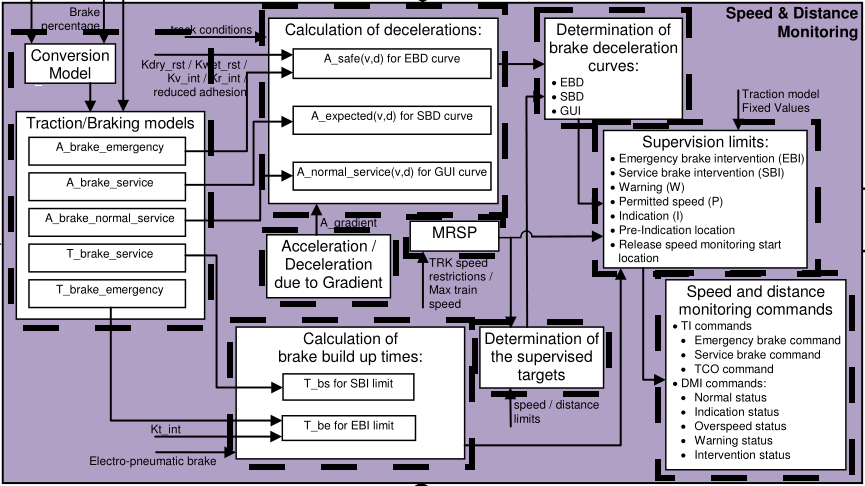
\includegraphics[width=.66\textwidth]{OverviewSelected}
  \caption{Decomposition of System}
  \label{fig:system-decomposition}
\end{figure}

Each of the sub-machines with its shared variables is then further refined until
the desired level of detail is reached. The overview of these refinements is
shown in Fig.~\ref{fig:machine-decompositon-overview}.

\begin{figure}[ht]
  \centering
  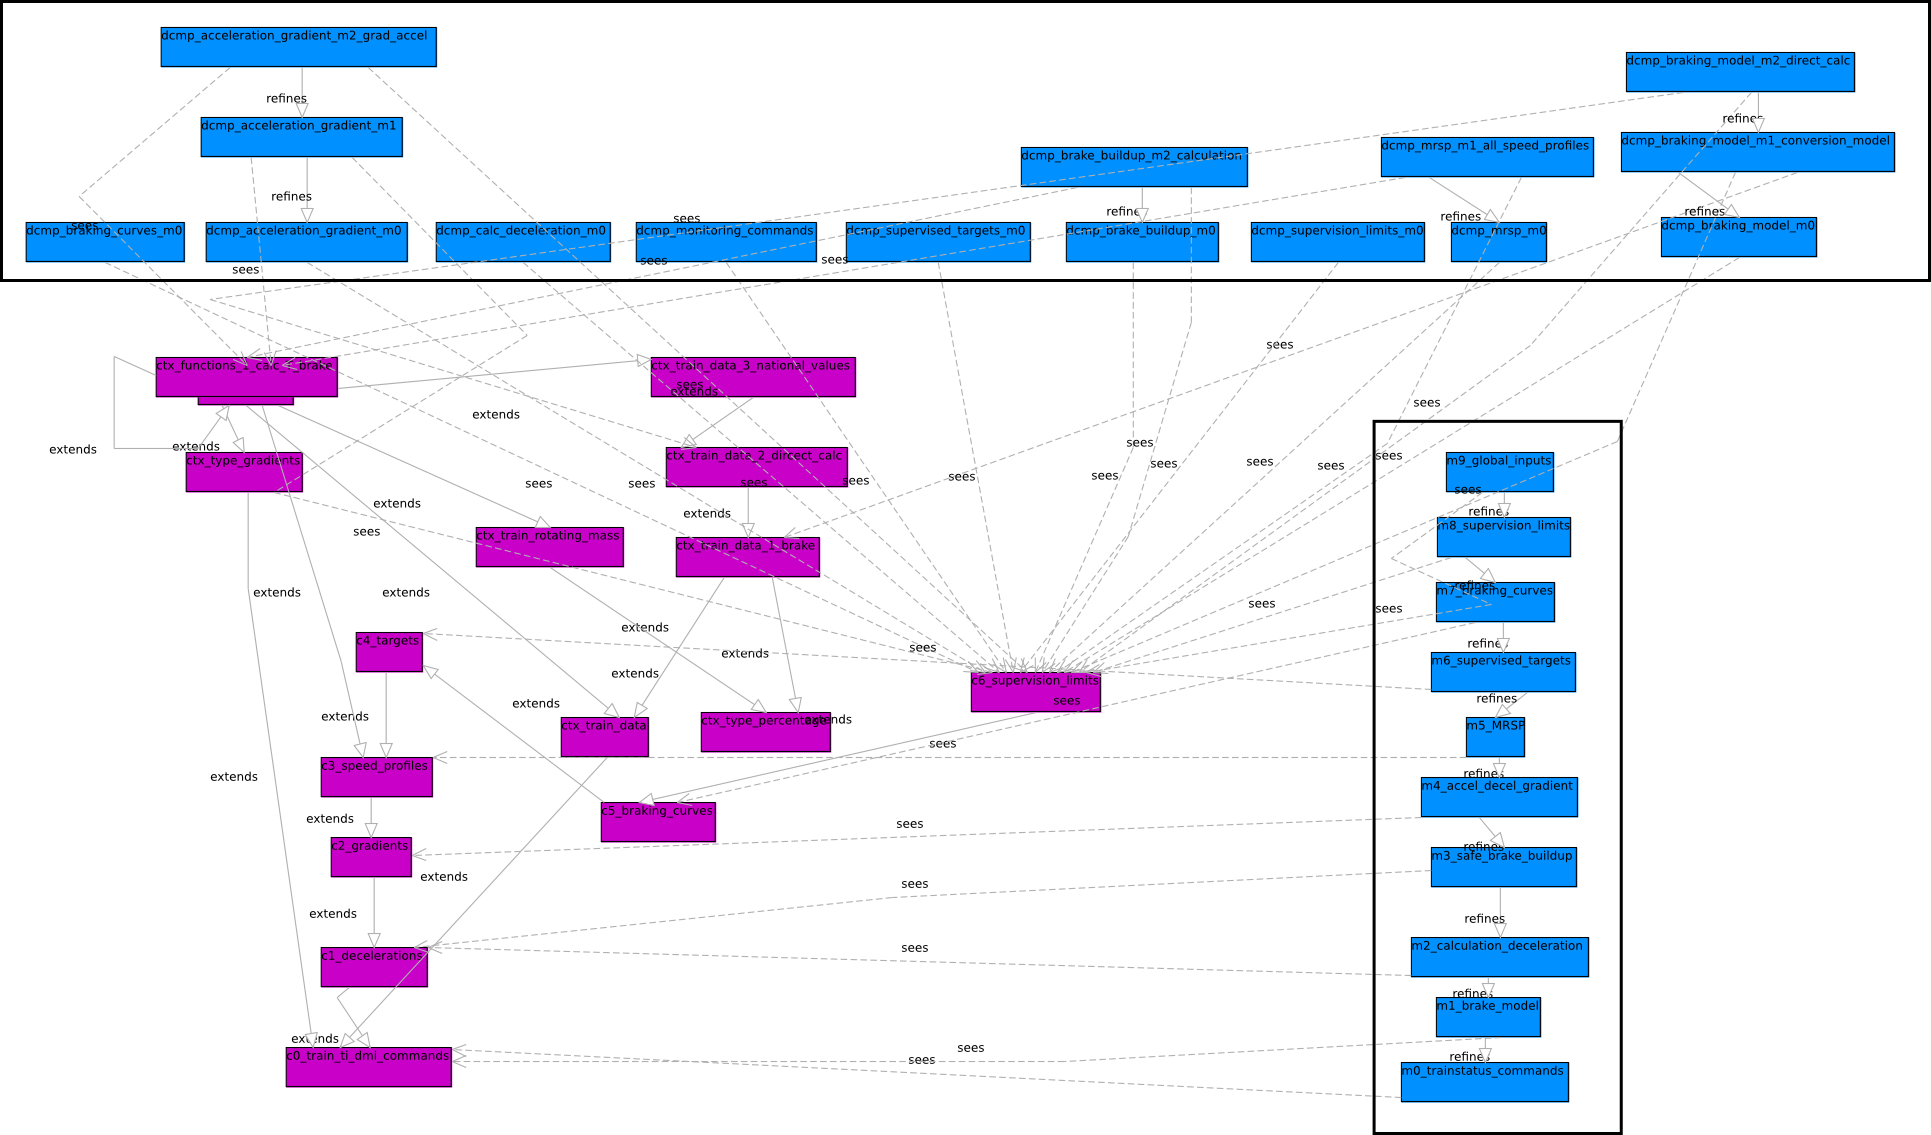
\includegraphics[width=\textwidth]{Section_3_13-layout}
  \caption{Machine Decomposition Overview}
  \label{fig:machine-decompositon-overview}
\end{figure}

This refinement and context overview is very different from the others, as first
an abstract global model was developed and then this model was decomposed into
sub-models which are further refined. The contexts are shared between the
decomposed models as far as possible. In this case, all resulting contexts and
machines are kept in the same Rodin project. It is also possible to create
a new project for each sub-machine which will reduce the complexity of each
single project.

The global model is shown in the lower right. The first machine describes the
global input and output variables of the system. The further refinements
represent the iterative addition of more functions as shown in
Fig.~\ref{fig:system-decomposition}. For example the machine 1 adds the brake
model with its inputs and outputs and the machine 2 adds the calculation of
deceleration which uses the outputs of the braking model.

The last machine is then decomposed into the nine machines representing each a
single functional block. This structure is shown in the upper part of
Fig.~\ref{fig:machine-decompositon-overview}, this also illustrates the further
independent refinement of the decomposed sub-machine.

The context hierarchy also reflects this structuring. The contexts define the
data types for the intermediate values, as well as the functions that calculate
these values. These functions are generally not further refined in the Event-B
model, as this is not part of the system modeling.

\section{Model Benefits}
\label{sec:model-highlights}

The modeled section of the SRS provides many details for calculation of various
values. The main content from a system modeling point of view is the model. So
while in this case the same benefits from using Rodin as
for~\cite{Section-3-5-Rodin,Section-4-6-Rodin,Section-5-9-Rodin} are present,
the main advantage here is the model structuring facility.

\begin{itemize}
\item {\bf Model Decomposition} The shared variable model
  decomposition~\cite{silva2011decomposition} allows for decomposing an Event-B
  model and for separate refining of the machines of the resulting
  sub-models while retaining correctness of the refinement proofs.
\end{itemize}

\section{Detailed Model Description}
\label{sec:deta-model-descr}


\subsection{Context 0 - Train Inputs, TI and DMI command}
\label{sec:context-0-entities}

The first context introduces many basic type for the model,
\btype{t\_locations}, \btype{t\_speed}, \btype{t\_acceleration},
\btype{t\_TI\_commands}, \btype{t\_DMI\_commands}, \btype{t\_time} and
\btype{t\_train\_modes}.

The commands for the train interface (TI) are represented by the constants
\bconst{c\_emergency\_brake}, \bconst{c\_service\_brake}, \bconst{c\_TCO},
\bconst{c\_no\_command}. For the driver machine interface (DMI) the commands are
represented by the constants \bconst{c\_normal}, \bconst{c\_indication},
\bconst{c\_overspeed}, \bconst{c\_warning} and \bconst{c\_intervention}.

The other constants provide default values for the initialization of variables
of that type.

{\footnotesize
\begin{description}
\CONTEXT{c0\_train\_ti\_dmi\_commands}
\SETS
        \begin{description}
                \ItemY{ t\_locations }{all possible locations on track }
                \ItemY{ t\_speed }{train speed measurement }
                \ItemY{ t\_acceleration }{train acceleration }
                \ItemY{ t\_TI\_commands }{track interface commands }
                \ItemY{ t\_DMI\_commands }{driver machine interface commands }
                \ItemY{ t\_time }{ }
                \Item{ t\_train\_modes }
        \end{description}
\CONSTANTS
        \begin{description}
                \Item{ c\_emergency\_brake }
                \Item{ c\_service\_brake }
                \ItemY{ c\_TCO }{traction cut off}
                \ItemY{ c\_no\_command }{empty command}
                \Item{ c\_normal }
                \Item{ c\_indication }
                \ItemY{ c\_overspeed }{}
                \ItemY{ c\_warning }{}
                \ItemY{ c\_intervention }{}
                \Item{ c\_v0 }
                \Item{ c\_a0 }
                \ItemY{ c\_l0 }{}
                \Item{ c\_a\_brake0 }
                \ItemY{ c\_T\_brake0 }{}
        \end{description}
\AXIOMS
        \begin{description}
                \nItem{ axm1 }{ partition(t\_TI\_commands,\{ c\_no\_command\}
                  ,\{ c\_emergency\_brake\} ,\\ \hspace*{1.2cm} \{ c\_service\_brake\} ,\{ c\_TCO\} ) }\cmt{ }
                \nItem{ axm2 }{ partition(t\_DMI\_commands,\{ c\_normal\} ,\{
                  c\_indication\},\\ \hspace*{1.2cm}\{ c\_overspeed\} ,\{ c\_warning\} ,\{ c\_intervention\} ) }		\nItem{ axm3 }{ c\_v0 \in  t\_speed }		\nItem{ axm4 }{ c\_a0 \in  t\_acceleration }\cmt{ }
                \nItem{ axm5 }{ c\_l0 \in  t\_locations }		\nItem{ axm6 }{ c\_a\_brake0 \in  t\_speed \tfun  t\_acceleration }\cmt{		\\\hspace*{1,4 cm}  default brake profile }
                \nItem{ axm7 }{ c\_T\_brake0 \in  t\_time }\cmt{		\\\hspace*{1,4 cm}  default brake buildup time }
        \end{description}
\END
\end{description}

}

\subsection{Machine 0 - Train Status and Commands}
\label{sec:machine-0-train}

This first machine introduces the external input variables, i.e., the position,
speed and acceleration of the train as well as the output variables, i.e., the
TI commands and the DMI commands. The input variables are read by the event
\bevent{update\_train\_style} and the output variables by the event
\bevent{new\_outputs}.

{\footnotesize
\begin{description}
\MACHINE{m0\_trainstatus\_commands}
\SEES{c0\_train\_ti\_dmi\_commands}
\VARIABLES
        \begin{description}
                \ItemY{ v\_current }{current speed of train}
                \ItemY{ a\_current }{current acceleration of train}
                \ItemY{ loc\_current }{current position of train as track location}
                \ItemY{ cmd\_current }{current TI command}
                \ItemY{ status\_current }{current DMI status}
        \end{description}
\INVARIANTS
        \begin{description}
                \nItem{ inv1 }{ v\_current \in  t\_speed }
                \nItem{ inv2 }{ a\_current \in  t\_acceleration }
                \nItemY{ inv3 }{ loc\_current \in  t\_locations }{  }
                \nItem{ inv4 }{ cmd\_current \in  t\_TI\_commands }
                \nItemY{ inv5 }{ status\_current \in  t\_DMI\_commands }{  }
        \end{description}
\EVENTS
        \INITIALISATION
                \begin{description}
                \BeginAct
                        \begin{description}
                        \nItem{ act1 }{ v\_current :=  c\_v0 }
                        \nItem{ act2 }{ a\_current :=  c\_a0 }
                        \nItemY{ act3 }{ loc\_current :=  c\_l0 }{  }
                        \nItemY{ act4 }{ cmd\_current :=  c\_no\_command }{  }
                        \nItemY{ act5 }{ status\_current :=  c\_normal }{  }
                        \end{description}
                \EndAct
                \end{description}
        \EVT {update\_train\_state}
                \begin{description}
                \AnyPrm
                        \begin{description}
                        \Item{l\_speed }
                        \Item{l\_accel }
                        \Item{l\_loc }
                        \end{description}
                \WhereGrd
                        \begin{description}
                        \nItem{ grd1 }{ l\_speed \in  t\_speed }
                        \nItem{ grd2 }{ l\_accel \in  t\_acceleration }
                        \nItemY{ grd3 }{ l\_loc \in  t\_locations }{ }
                        \end{description}
                \ThenAct
                        \begin{description}
                        \nItem{ act1 }{ v\_current :=  l\_speed }
                        \nItem{ act2 }{ a\_current :=  l\_accel }
                        \nItem{ act3 }{ loc\_current :=  l\_loc }
                        \end{description}
                \EndAct
                \end{description}
        \EVT {new\_outputs}
                \begin{description}
                \AnyPrm
                        \begin{description}
                        \Item{l\_ti\_cmd }
                        \Item{l\_dmi\_status }
                        \end{description}
                \WhereGrd
                        \begin{description}
                        \nItemY{ grd1 }{ l\_ti\_cmd \in  t\_TI\_commands }{ }
                        \nItemY{ grd2 }{ l\_dmi\_status \in  t\_DMI\_commands }{ }
                        \end{description}
                \ThenAct
                        \begin{description}
                        \nItemY{ act1 }{ cmd\_current :=  l\_ti\_cmd }{  }
                        \nItem{ act2 }{ status\_current :=  l\_dmi\_status }
                        \end{description}
                \EndAct
                \end{description}
\END
\end{description}

}

\subsection{Machine 1 - Brake Model}
\label{sec:machine-1-brake}

The first refinement adds the notion of the brake model. This is represented by
the variables describing the speed dependent acceleration functions for
emergency, service and normal service braking. The variables
\bvar{T\_brake\_service} and \bvar{T\_brake\_emergency} describe the brake
build-up times for the brakes.

{\footnotesize
\begin{description}
\MACHINE{m1\_brake\_model}
\REFINES{m0\_trainstatus\_commands}
\SEES{c0\_train\_ti\_dmi\_commands}
\VARIABLES
        \begin{description}
                \ItemY{ A\_brake\_emergency }{emergency brake acceleration}
                \ItemY{ A\_brake\_service }{service brake acceleration}
                \Item{ A\_brake\_normal\_service }
                \Item{ T\_brake\_service }
                \Item{ T\_brake\_emergency }
        \end{description}
\EVENTS
        \EVT {set\_A\_brake\_emergency}
                \begin{description}
                \AnyPrm
                        \begin{description}
                        \Item{l\_a\_brake }
                        \end{description}
                \WhereGrd
                        \begin{description}
                        \nItemY{ grd1 }{ l\_a\_brake \in  t\_speed \tfun  t\_acceleration }{ }
                        \end{description}
                \ThenAct
                        \begin{description}
                        \nItem{ act1 }{ A\_brake\_emergency :=  l\_a\_brake }
                        \end{description}
                \EndAct
                \end{description}
        \EVT {set\_A\_brake\_service}
                \begin{description}
                \AnyPrm
                        \begin{description}
                        \Item{l\_a\_brake }
                        \end{description}
                \WhereGrd
                        \begin{description}
                        \nItem{ grd1 }{ l\_a\_brake \in  t\_speed \tfun  t\_acceleration }
                        \end{description}
                \ThenAct
                        \begin{description}
                        \nItem{ act1 }{ A\_brake\_service :=  l\_a\_brake }
                        \end{description}
                \EndAct
                \end{description}
        \EVT {set\_A\_brake\_normal\_service}
                \begin{description}
                \AnyPrm
                        \begin{description}
                        \Item{l\_a\_brake }
                        \end{description}
                \WhereGrd
                        \begin{description}
                        \nItem{ grd1 }{ l\_a\_brake \in  t\_speed \tfun  t\_acceleration }
                        \end{description}
                \ThenAct
                        \begin{description}
                        \nItem{ act1 }{ A\_brake\_normal\_service :=  l\_a\_brake }
                        \end{description}
                \EndAct
                \end{description}
        \EVT {set\_T\_brake\_service}
                \begin{description}
                \AnyPrm
                        \begin{description}
                        \Item{l\_T\_brake }
                        \end{description}
                \WhereGrd
                        \begin{description}
                        \nItem{ grd1 }{ l\_T\_brake \in  t\_time }
                        \end{description}
                \ThenAct
                        \begin{description}
                        \nItem{ act1 }{ T\_brake\_service :=  l\_T\_brake }
                        \end{description}
                \EndAct
                \end{description}
        \EVT {set\_T\_brake\_emergency}
                \begin{description}
                \AnyPrm
                        \begin{description}
                        \Item{l\_T\_brake }
                        \end{description}
                \WhereGrd
                        \begin{description}
                        \nItem{ grd1 }{ l\_T\_brake \in  t\_time }
                        \end{description}
                \ThenAct
                        \begin{description}
                        \nItem{ act1 }{ T\_brake\_emergency :=  l\_T\_brake }
                        \end{description}
                \EndAct
                \end{description}
\END
\end{description}

}

\subsection{Context 1 - Decelerations}
\label{sec:cont-1-decel}

This context extension adds a distance type and a function that maps the speed
and distance to an acceleration.

{\footnotesize
\begin{description}
\CONTEXT{c1\_decelerations}
\EXTENDS{c0\_train\_ti\_dmi\_commands}
\SETS
        \begin{description}
                \Item{ t\_distance }
        \end{description}
\CONSTANTS
        \begin{description}
                \Item{ f\_A\_deceleration0 }
        \end{description}
\AXIOMS
        \begin{description}
                \nItem{ axm1 }{ f\_A\_deceleration0 \in  t\_speed \cprod  t\_distance \tfun  t\_acceleration }	\end{description}
\END
\end{description}

}

\subsection{Machine 2 - Calculate Decelerations}
\label{sec:machine-2-calculate}

This refinement adds the calculation of deceleration to the model. This is
represented by three variables which are functions that map speed and distance
to an acceleration. There is one function for each on of EBD, SBD and GUI.

{\footnotesize
\begin{description}
\MACHINE{m2\_calculation\_deceleration}
\REFINES{m1\_brake\_model}
\SEES{c1\_decelerations}
\VARIABLES
        \begin{description}
                \Item{ A\_safe }
                \Item{ A\_expected }
                \ItemY{ A\_normal\_service }{}
        \end{description}
\EVENTS
        \EVT {set\_A\_safe}
                \begin{description}
                \AnyPrm
                        \begin{description}
                        \Item{l\_a\_decel }
                        \end{description}
                \WhereGrd
                        \begin{description}
                        \nItemY{ grd1 }{ l\_a\_decel \in  t\_speed \cprod  t\_distance \tfun  t\_acceleration }{ }
                        \nItem{ grd2 }{ A\_brake\_emergency \in  t\_speed \tfun  t\_acceleration }
                        \end{description}
                \ThenAct
                        \begin{description}
                        \nItem{ act1 }{ A\_safe :=  l\_a\_decel }
                        \end{description}
                \EndAct
                \end{description}
        \EVT {set\_A\_expected}
                \begin{description}
                \AnyPrm
                        \begin{description}
                        \Item{l\_a\_decel }
                        \end{description}
                \WhereGrd
                        \begin{description}
                        \nItemY{ grd1 }{ l\_a\_decel \in  t\_speed \cprod  t\_distance \tfun  t\_acceleration }{ }
                        \nItem{ grd2 }{ A\_brake\_service \in  t\_speed \tfun  t\_acceleration }
                        \end{description}
                \ThenAct
                        \begin{description}
                        \nItem{ act1 }{ A\_expected :=  l\_a\_decel }
                        \end{description}
                \EndAct
                \end{description}
        \EVT {set\_A\_normal\_service}
                \begin{description}
                \AnyPrm
                        \begin{description}
                        \Item{l\_a\_decel }
                        \end{description}
                \WhereGrd
                        \begin{description}
                        \nItemY{ grd1 }{ l\_a\_decel \in  t\_speed \cprod  t\_distance \tfun  t\_acceleration }{ }
                        \nItem{ grd2 }{ A\_brake\_normal\_service \in  t\_speed \tfun  t\_acceleration }
                        \end{description}
                \ThenAct
                        \begin{description}
                        \nItem{ act1 }{ A\_normal\_service :=  l\_a\_decel }
                        \end{description}
                \EndAct
                \end{description}
\END
\end{description}

}

\subsection{Machine 3 - Calculation of Brake Buildup Time}
\label{sec:mach-3-calc}

The next machine refinement adds the brake buildup calculation to the
model. This is represented by two variables, \bvar{T\_be} for the emergency
brake and \bvar{T\_se} for the service brake.

{\footnotesize
\begin{description}
\MACHINE{m3\_safe\_brake\_buildup}
\REFINES{m2\_calculation\_deceleration}
\SEES{c1\_decelerations}
\VARIABLES
        \begin{description}
                \ItemY{ T\_be }{}
                \Item{ T\_bs }
        \end{description}
\EVENTS
        \EVT {set\_T\_be}
                \begin{description}
                \AnyPrm
                        \begin{description}
                        \Item{l\_t\_be }
                        \end{description}
                \WhereGrd
                        \begin{description}
                        \nItemY{ grd1 }{ l\_t\_be \in  t\_time }{ }
                        \nItem{ grd2 }{ T\_brake\_emergency \in  t\_time }
                        \end{description}
                \ThenAct
                        \begin{description}
                        \nItem{ act1 }{ T\_be :=  l\_t\_be }
                        \end{description}
                \EndAct
                \end{description}
        \EVT {set\_T\_bs}
                \begin{description}
                \AnyPrm
                        \begin{description}
                        \Item{l\_t\_bs }
                        \end{description}
                \WhereGrd
                        \begin{description}
                        \nItemY{ grd1 }{ l\_t\_bs \in  t\_time }{ }
                        \nItem{ grd2 }{ T\_brake\_service \in  t\_time }
                        \end{description}
                \ThenAct
                        \begin{description}
                        \nItem{ act1 }{ T\_bs :=  l\_t\_bs }
                        \end{description}
                \EndAct
                \end{description}
\END
\end{description}

}

\subsection{Machine 4 - Acceleration due to Gradient}
\label{sec:mach-4-accel}

The refinement adds the notion of the acceleration due to gradient. This is
represented by the variable \bvar{A\_gradient} which is a function that maps
speed to acceleration.

{\footnotesize
\begin{description}
\MACHINE{m4\_accel\_decel\_gradient}
\REFINES{m3\_safe\_brake\_buildup}
\SEES{c2\_gradients}
\VARIABLES
        \begin{description}
                \Item{ A\_gradient }
        \end{description}

\EVENTS
        \EVT {set\_A\_gradient}
                \begin{description}
                \AnyPrm
                        \begin{description}
                        \Item{l\_a\_gradient }
                        \end{description}
                \WhereGrd
                        \begin{description}
                        \nItem{ grd1 }{ l\_a\_gradient \in  t\_acceleration }
                        \end{description}
                \ThenAct
                        \begin{description}
                        \nItem{ act1 }{ A\_gradient :=  l\_a\_gradient }
                        \end{description}
                \EndAct
                \end{description}
\END
\end{description}

}

\subsection{Context 3 - Speed Profiles}
\label{sec:context-3-speed}

This context extension introduces the type \btype{speed\_profiles} which maps
locations to speeds. It also defines one constant value of that type which is
used as default value for variables of that type.

{\footnotesize
\begin{description}
\CONTEXT{c3\_speed\_profiles}
\EXTENDS{c2\_gradients}
\CONSTANTS
        \begin{description}
                \Item{ c\_speed\_profile0 }
                \Item{ t\_speed\_profiles }
        \end{description}
\AXIOMS
        \begin{description}
                \nItem{ axm1 }{ t\_speed\_profiles \subseteq  t\_locations \cprod  t\_speed }		\nItem{ axm2 }{ c\_speed\_profile0 \in  t\_speed\_profiles }	\end{description}
\END
\end{description}

}

\subsection{Machine 5 - Most Restrictive Speed Profile}
\label{sec:machine-5-most}

This machine refinement introduces the most restrictive speed profile to the
model. This is represented by the variable \bvar{MRSP} of the type
\btype{speed\_profile}.

{\footnotesize
\begin{description}
\MACHINE{m5\_MRSP}
\REFINES{m4\_accel\_decel\_gradient}
\SEES{c3\_speed\_profiles}
\VARIABLES
        \begin{description}
                \Item{ MRSP }
        \end{description}
\EVENTS
        \EVT {set\_MRSP}
                \begin{description}
                \AnyPrm
                        \begin{description}
                        \Item{l\_sp }
                        \end{description}
                \WhereGrd
                        \begin{description}
                        \nItemY{ grd1 }{ l\_sp \in  t\_speed\_profiles }{ }
                        \end{description}
                \ThenAct
                        \begin{description}
                        \nItem{ act1 }{ MRSP :=  l\_sp }
                        \end{description}
                \EndAct
                \end{description}
\END
\end{description}

}

\subsection{Context 4 - Targets}
\label{sec:context-4-targets}

This context extension introduces the type \btype{t\_targets} which represents a
target, i.e., a pair of location and speed.

{\footnotesize
\begin{description}
\CONTEXT{c4\_targets}
\EXTENDS{c3\_speed\_profiles}
\CONSTANTS
        \begin{description}
                \Item{ t\_targets }
                \Item{ c\_target0 }
        \end{description}
\AXIOMS
        \begin{description}
                \nItem{ axm1 }{ t\_targets \subseteq  t\_locations \cprod  t\_speed }\cmt{ }
                \nItem{ axm2 }{ c\_target0 \in  t\_targets }	\end{description}
\END
\end{description}

}

\subsection{Machine 6 - Supervised Targets}
\label{sec:machine-6-supervised}

This refinement adds limit of authority, end of authority and supervision limit
to the model. For each there exists one variable of type \btype{t\_targets}.

{\footnotesize
\begin{description}
\MACHINE{m6\_supervised\_targets}
\REFINES{m5\_MRSP}
\SEES{c4\_targets}
\VARIABLES
        \begin{description}
                \Item{ LOA }
                \Item{ EOA }
                \Item{ SvL }
        \end{description}
\EVENTS
        \EVT {set\_EOA}
                \begin{description}
                \AnyPrm
                        \begin{description}
                        \Item{l\_target }
                        \end{description}
                \WhereGrd
                        \begin{description}
                        \nItemY{ grd1 }{ l\_target \in  t\_targets }{ }
                        \nItem{ grd2 }{ MRSP \in  t\_speed\_profiles }
                        \end{description}
                \ThenAct
                        \begin{description}
                        \nItem{ act1 }{ EOA :=  l\_target }
                        \end{description}
                \EndAct
                \end{description}
        \EVT {set\_LOA}
                \begin{description}
                \AnyPrm
                        \begin{description}
                        \Item{l\_target }
                        \end{description}
                \WhereGrd
                        \begin{description}
                        \nItem{ grd1 }{ l\_target \in  t\_targets }
                        \nItem{ grd2 }{ MRSP \in  t\_speed\_profiles }
                        \end{description}
                \ThenAct
                        \begin{description}
                        \nItem{ act1 }{ LOA :=  l\_target }
                        \end{description}
                \EndAct
                \end{description}
        \EVT {set\_SvL}
                \begin{description}
                \AnyPrm
                        \begin{description}
                        \Item{l\_target }
                        \end{description}
                \WhereGrd
                        \begin{description}
                        \nItemY{ grd1 }{ l\_target \in  t\_targets }{ }
                        \nItem{ grd2 }{ MRSP \in  t\_speed\_profiles }
                        \end{description}
                \ThenAct
                        \begin{description}
                        \nItem{ act1 }{ SvL :=  l\_target }
                        \end{description}
                \EndAct
                \end{description}
\END
\end{description}

}

\subsection{Context 5 - Braking Curves}
\label{sec:context-5-braking}

This context extension introduces the type \btype{t\_braking\_curves} and a
constant of that type.

{\footnotesize
\begin{description}
\CONTEXT{c5\_braking\_curves}
\EXTENDS{c4\_targets}
\SETS
        \begin{description}
                \Item{ t\_braking\_curves }
        \end{description}
\CONSTANTS
        \begin{description}
                \Item{ c\_curve0 }
        \end{description}
\AXIOMS
        \begin{description}
                \nItem{ axm1 }{ c\_curve0 \in  t\_braking\_curves }	\end{description}
\END
\end{description}



\subsection{Machine 7 - Braking Curves}
\label{sec:machine-7-braking}

This machine refinement adds the braking curves to the model, these are
represented by the three variables \bvar{EBD}, \bvar{SBD} and \bvar{GUI} of the
appropriate type.

{\footnotesize
\begin{description}
\MACHINE{m7\_braking\_curves}
\REFINES{m6\_supervised\_targets}
\SEES{c5\_braking\_curves}
\VARIABLES
        \begin{description}
                \Item{ EBD }
                \Item{ SBD }
                \Item{ GUI }
        \end{description}
\EVENTS
        \EVT {set\_EBD}
                \begin{description}
                \AnyPrm
                        \begin{description}
                        \Item{l\_curve }
                        \end{description}
                \WhereGrd
                        \begin{description}
                        \nItemY{ grd1 }{ l\_curve \in  t\_braking\_curves }{ }
                        \nItemY{ grd2 }{ A\_safe \in  t\_speed \cprod  t\_distance \tfun  t\_acceleration }{ }
                        \nItem{ grd3 }{ A\_expected \in  t\_speed \cprod  t\_distance \tfun  t\_acceleration }
                        \nItemY{ grd4 }{ A\_normal\_service \in  t\_speed \cprod  t\_distance \tfun  t\_acceleration }{ }
                        \nItem{ grd5 }{ LOA \in  t\_targets }
                        \nItem{ grd6 }{ EOA \in  t\_targets }
                        \nItem{ grd7 }{ SvL \in  t\_targets }
                        \end{description}
                \ThenAct
                        \begin{description}
                        \nItem{ act1 }{ EBD :=  l\_curve }
                        \end{description}
                \EndAct
                \end{description}
        \EVT {set\_SBD}
                \begin{description}
                \AnyPrm
                        \begin{description}
                        \Item{l\_curve }
                        \end{description}
                \WhereGrd
                        \begin{description}
                        \nItemY{ grd1 }{ l\_curve \in  t\_braking\_curves }{ }
                        \nItemY{ grd2 }{ A\_safe \in  t\_speed \cprod  t\_distance \tfun  t\_acceleration }{ }
                        \nItemY{ grd3 }{ A\_expected \in  t\_speed \cprod  t\_distance \tfun  t\_acceleration }{ }
                        \nItemY{ grd4 }{ A\_normal\_service \in  t\_speed \cprod  t\_distance \tfun  t\_acceleration }{ }
                        \nItem{ grd5 }{ LOA \in  t\_targets }
                        \nItem{ grd6 }{ EOA \in  t\_targets }
                        \nItem{ grd7 }{ SvL \in  t\_targets }
                        \end{description}
                \ThenAct
                        \begin{description}
                        \nItem{ act1 }{ SBD :=  l\_curve }
                        \end{description}
                \EndAct
                \end{description}
        \EVT {set\_GUI}
                \begin{description}
                \AnyPrm
                        \begin{description}
                        \Item{l\_curve }
                        \end{description}
                \WhereGrd
                        \begin{description}
                        \nItem{ grd1 }{ l\_curve \in  t\_braking\_curves }
                        \nItem{ grd2 }{ A\_safe \in  t\_speed \cprod  t\_distance \tfun  t\_acceleration }
                        \nItem{ grd3 }{ A\_expected \in  t\_speed \cprod  t\_distance \tfun  t\_acceleration }
                        \nItemY{ grd4 }{ A\_normal\_service \in  t\_speed \cprod  t\_distance \tfun  t\_acceleration }{ }
                        \nItem{ grd5 }{ LOA \in  t\_targets }
                        \nItem{ grd6 }{ EOA \in  t\_targets }
                        \nItem{ grd7 }{ SvL \in  t\_targets }
                        \end{description}
                \ThenAct
                        \begin{description}
                        \nItem{ act1 }{ GUI :=  l\_curve }
                        \end{description}
                \EndAct
                \end{description}
\END
\end{description}

}

\subsection{Context 6 - Supervision Limits}
\label{sec:cont-6-superv}

This context adds the type \btype{t\_supervision\_limits} to the model, as well
as a constant value of that type.

{\footnotesize
\begin{description}
\CONTEXT{c6\_supervision\_limits}
\EXTENDS{c5\_braking\_curves}
\SETS
        \begin{description}
                \Item{ t\_supervision\_limits }
        \end{description}
\CONSTANTS
        \begin{description}
                \Item{ c\_slimit0 }
        \end{description}
\AXIOMS
        \begin{description}
                \nItem{ axm1 }{ c\_slimit0 \in  t\_supervision\_limits }	\end{description}
\END
\end{description}

}

\subsection{Machine 8 - Supervision Limit}
\label{sec:mach-8-superv}

This machine refinement adds the supervision limits to the model, emergency
brake intervention (\bvar{EBI}), service brake intervention (\bvar{SBI}),
warning limit (\bvar{warning\_limit}), permitted speed (\bvar{P\_limit}),
indication limit (\bvar{I\_limit}), pre-indication location (\bvar{PI\_limit})
and the release start speed monitoring location (\bvar{RSM\_start}).

{\footnotesize
\begin{description}
\MACHINE{m8\_supervision\_limits}
\REFINES{m7\_braking\_curves}
\SEES{c6\_supervision\_limits}
\VARIABLES
        \begin{description}
                \ItemY{ EBI }{emergency brake intervention}
                \ItemY{ SBI }{service brake intervention}
                \ItemY{ W\_limit }{warning limit}
                \ItemY{ P\_limit }{permitted speed}
                \ItemY{ I\_limit }{indication limit}
                \ItemY{ PIl }{pre-indication$\_$location}
                \ItemY{ RSM\_start }{release speed monitoring start location}
        \end{description}
\EVENTS
        \EVT {set\_EBI}
                \begin{description}
                \AnyPrm
                        \begin{description}
                        \ItemY{l\_limit }{ }
                        \end{description}
                \WhereGrd
                        \begin{description}
                        \nItemY{ grd1 }{ l\_limit \in  t\_supervision\_limits }{ }
                        \nItemY{ grd2 }{ MRSP \in  t\_speed\_profiles }{ }
                        \nItem{ grd3 }{ EBD \in  t\_braking\_curves }
                        \nItem{ grd4 }{ SBD \in  t\_braking\_curves }
                        \nItem{ grd5 }{ GUI \in  t\_braking\_curves }
                        \nItem{ grd6 }{ T\_bs \in  t\_time }
                        \nItem{ grd7 }{ T\_be \in  t\_time }
                        \end{description}
                \ThenAct
                        \begin{description}
                        \nItem{ act1 }{ EBI :=  l\_limit }
                        \end{description}
                \EndAct
                \end{description}
        \EVT {set\_SBI}\cmt{ }
                \begin{description}
                \AnyPrm
                        \begin{description}
                        \ItemY{l\_limit }{ }
                        \end{description}
                \WhereGrd
                        \begin{description}
                        \nItemY{ grd1 }{ l\_limit \in  t\_supervision\_limits }{ }
                        \nItemY{ grd2 }{ MRSP \in  t\_speed\_profiles }{ }
                        \nItem{ grd3 }{ EBD \in  t\_braking\_curves }
                        \nItem{ grd4 }{ SBD \in  t\_braking\_curves }
                        \nItem{ grd5 }{ GUI \in  t\_braking\_curves }
                        \nItem{ grd6 }{ T\_bs \in  t\_time }
                        \nItem{ grd7 }{ T\_be \in  t\_time }
                        \end{description}
                \ThenAct
                        \begin{description}
                        \nItem{ act1 }{ SBI :=  l\_limit }
                        \end{description}
                \EndAct
                \end{description}
        \EVT {set\_W\_limit}\cmt{ }
                \begin{description}
                \AnyPrm
                        \begin{description}
                        \ItemY{l\_limit }{ }
                        \end{description}
                \WhereGrd
                        \begin{description}
                        \nItem{ grd1 }{ l\_limit \in  t\_supervision\_limits }
                        \nItemY{ grd2 }{ MRSP \in  t\_speed\_profiles }{ }
                        \nItem{ grd3 }{ EBD \in  t\_braking\_curves }
                        \nItem{ grd4 }{ SBD \in  t\_braking\_curves }
                        \nItem{ grd5 }{ GUI \in  t\_braking\_curves }
                        \nItem{ grd6 }{ T\_bs \in  t\_time }
                        \nItem{ grd7 }{ T\_be \in  t\_time }
                        \end{description}
                \ThenAct
                        \begin{description}
                        \nItem{ act1 }{ W\_limit :=  l\_limit }
                        \end{description}
                \EndAct
                \end{description}
        \EVT {set\_I\_limit}\cmt{ }
                \begin{description}
                \AnyPrm
                        \begin{description}
                        \ItemY{l\_limit }{ }
                        \end{description}
                \WhereGrd
                        \begin{description}
                        \nItem{ grd1 }{ l\_limit \in  t\_supervision\_limits }
                        \nItemY{ grd2 }{ MRSP \in  t\_speed\_profiles }{ }
                        \nItem{ grd3 }{ EBD \in  t\_braking\_curves }
                        \nItem{ grd4 }{ SBD \in  t\_braking\_curves }
                        \nItem{ grd5 }{ GUI \in  t\_braking\_curves }
                        \nItem{ grd6 }{ T\_bs \in  t\_time }
                        \nItem{ grd7 }{ T\_be \in  t\_time }
                        \end{description}
                \ThenAct
                        \begin{description}
                        \nItem{ act1 }{ I\_limit :=  l\_limit }
                        \end{description}
                \EndAct
                \end{description}
        \EVT {set\_P\_limit}\cmt{ }
                \begin{description}
                \AnyPrm
                        \begin{description}
                        \ItemY{l\_limit }{ }
                        \end{description}
                \WhereGrd
                        \begin{description}
                        \nItem{ grd1 }{ l\_limit \in  t\_supervision\_limits }
                        \nItemY{ grd2 }{ MRSP \in  t\_speed\_profiles }{ }
                        \nItem{ grd3 }{ EBD \in  t\_braking\_curves }
                        \nItem{ grd4 }{ SBD \in  t\_braking\_curves }
                        \nItem{ grd5 }{ GUI \in  t\_braking\_curves }
                        \nItem{ grd6 }{ T\_bs \in  t\_time }
                        \nItem{ grd7 }{ T\_be \in  t\_time }
                        \end{description}
                \ThenAct
                        \begin{description}
                        \nItem{ act1 }{ P\_limit :=  l\_limit }
                        \end{description}
                \EndAct
                \end{description}
        \EVT {set\_PIl\_limit}\cmt{ }
                \begin{description}
                \AnyPrm
                        \begin{description}
                        \ItemY{l\_limit }{ }
                        \end{description}
                \WhereGrd
                        \begin{description}
                        \nItem{ grd1 }{ l\_limit \in  t\_supervision\_limits }
                        \nItemY{ grd2 }{ MRSP \in  t\_speed\_profiles }{ }
                        \nItem{ grd3 }{ EBD \in  t\_braking\_curves }
                        \nItem{ grd4 }{ SBD \in  t\_braking\_curves }
                        \nItem{ grd5 }{ GUI \in  t\_braking\_curves }
                        \nItem{ grd6 }{ T\_bs \in  t\_time }
                        \nItem{ grd7 }{ T\_be \in  t\_time }
                        \end{description}
                \ThenAct
                        \begin{description}
                        \nItem{ act1 }{ PIl :=  l\_limit }
                        \end{description}
                \EndAct
                \end{description}
        \EVT {set\_RSM\_start\_limit}\cmt{ }
                \begin{description}
                \AnyPrm
                        \begin{description}
                        \ItemY{l\_limit }{ }
                        \end{description}
                \WhereGrd
                        \begin{description}
                        \nItem{ grd1 }{ l\_limit \in  t\_supervision\_limits }
                        \nItemY{ grd2 }{ MRSP \in  t\_speed\_profiles }{ }
                        \nItem{ grd3 }{ EBD \in  t\_braking\_curves }
                        \nItem{ grd4 }{ SBD \in  t\_braking\_curves }
                        \nItem{ grd5 }{ GUI \in  t\_braking\_curves }
                        \nItem{ grd6 }{ T\_bs \in  t\_time }
                        \nItem{ grd7 }{ T\_be \in  t\_time }
                        \end{description}
                \ThenAct
                        \begin{description}
                        \nItem{ act1 }{ RSM\_start :=  l\_limit }
                        \end{description}
                \EndAct
                \end{description}
\END
\end{description}

}

\section{Model Decomposition}
\label{sec:model-decomposition}

The machine m9 does not really add detail to the refined machine m8. The only
changes are that the variables which are read by an event are explicitly added
to the conditions by specifying a typing condition for them. This assures that
the model decomposition preserves these necessary variables in the sub-machines
and only removes the unneeded ones.

\bibliographystyle{alpha}
\bibliography{openetcs}

\end{document}


%%% Local Variables:
%%% mode: latex
%%% TeX-master: t
%%% End:
